\section{ÔN TẬP CHƯƠNG 3}
\subsection{Câu trắc nghiệm nhiều phương án lựa chọn}
\textit{Thí sinh trả lời từ câu 1 đến câu 18. Mỗi câu thí sinh chọn một phương án}
\setcounter{ex}{0}
\Opensolutionfile{ans}[ans/VN12-Y24-PH-SYL-024-TN]
% ===================================================================
\begin{ex}
	Tương tác nào sau đây \textbf{không phải} là tương tác từ?
	\choice
	{Tương tác giữa hai dòng điện}
	{Tương tác giữa thanh sắt hút nam châm}
	{Tương tác giữa nam châm và dòng điện}
	{\True Tương tác giữa Trái Đất hút một nam châm}
	\loigiai{}
\end{ex}
% ===================================================================
\begin{ex}
	Cảm ứng từ của một dòng điện chạy trong dây dẫn thẳng dài tại một điểm M có độ lớn tăng khi
	\choice
	{M dịch chuyển theo một đường sức từ}
	{M dịch chuyển theo hướng vuông góc với dây và ra xa dây}
	{M dịch chuyển theo đường song song với dây}
	{\True M dịch chuyển theo hướng vuông góc với dây và lại gần đây}
	\loigiai{}
\end{ex}
% ===================================================================
\begin{ex}
	Từ trường \textbf{không} có xung quanh
	\choice
	{nam châm tự nhiên}
	{\True một điện tích đứng yên}
	{một đoạn dây dẫn có dòng điện}
	{nam châm điện}
	\loigiai{}
\end{ex}
% ===================================================================
\begin{ex}
	Một đoạn dây có dòng điện được đặt trong từ trường đều có vector cảm ứng từ $\vec{B}$. Để lực từ tác dụng lên dây cực đại thì góc $\alpha$ giữa dây dẫn và $\vec{B}$ phải bằng
	\choice
	{$\alpha=\SI{0}{\degree}$}
	{$\alpha=\SI{30}{\degree}$}
	{$\alpha=\SI{60}{\degree}$}
	{\True $\alpha=\SI{90}{\degree}$}
	\loigiai{
		Lực điện từ tác dụng lên đoạn dây dẫn chiều dài $\ell$ có dòng điện $I$ chạy qua được đặt trong một từ trường đều $\vec{B}$ và góc hợp với $\vec{B}$ là $\alpha$ bằng:
		$F=I\ell B\sin\alpha\Rightarrow F=F_\text{max}$ khi $\sin\alpha=1\Rightarrow\alpha=\SI{90}{\degree}.$
	}
\end{ex}
% ===================================================================
\begin{ex}
	Trong các hình vẽ sau về chiều của cảm ứng từ $B$, dòng điện $I$, lực từ $F$. Hình vẽ nào \textbf{đúng}?
	\begin{center}
		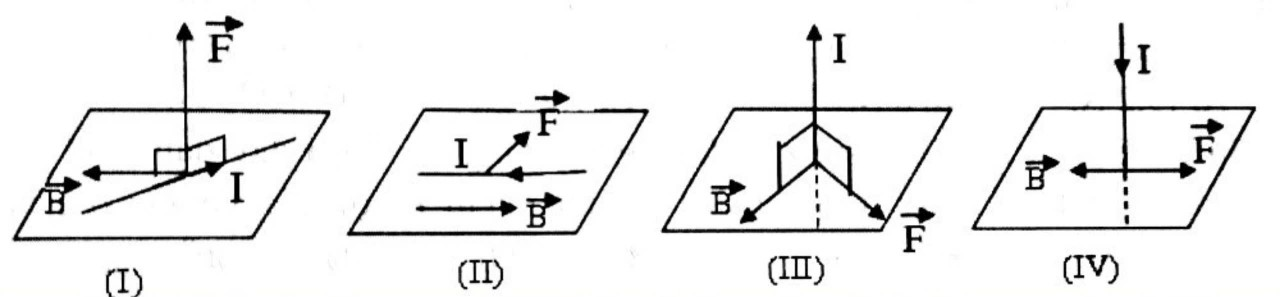
\includegraphics[width=0.7\linewidth]{figs/VN12-Y24-PH-SYL-025P-1}
	\end{center}
	\choice
	{Hình III}
	{Hình I, II}
	{\True Hình I, III}
	{Hình II, IV}
	\loigiai{}
\end{ex}
% ===================================================================
\begin{ex}
	Một đoạn dây dẫn thẳng dài $\SI{20}{\centi\meter}$ mang dòng điện $\SI{5}{\ampere}$ đặt trong từ trường đều có cảm ứng từ $B=\SI{0.3}{\tesla}$. Lực từ tác dụng lên đoạn dây có giá trị $\SI{0.15}{\newton}$. Đoạn dây hợp với vector cảm ứng từ một góc là
	\choice
	{$\SI{20}{\degree}$}
	{$\SI{25}{\degree}$}
	{\True $\SI{30}{\degree}$}
	{$\SI{45}{\degree}$}
	\loigiai{
		$\sin\alpha=\dfrac{F}{I\ell B}=0.5\Rightarrow \alpha=\SI{30}{\degree}.$	
	}
\end{ex}
% ===================================================================
\begin{ex}
	\immini{	Một dây dẫn thẳng mang dòng điện $I_1$ và một dây dẫn tròn mang dòng điện $I_2$ được bố trí trong không gian như hình bên. Trong những vùng không gian nào, vector cảm ứng từ do hai dòng điện gây ra có chiều ngược nhau?
	\choice
	{Vùng (1) và (3)}
	{\True Vùng (2) và (4)}
	{Vùng (1) và (4)}
	{Vùng (2) và (3)}}
	{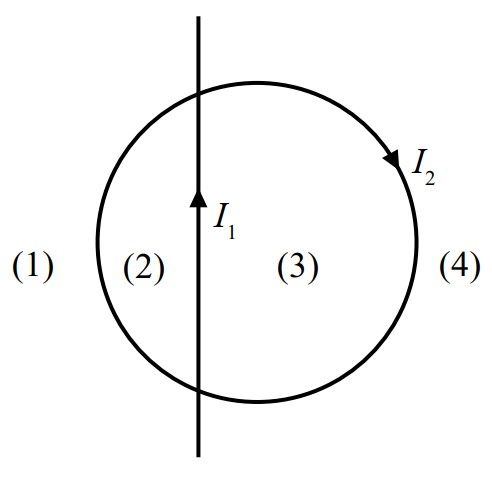
\includegraphics[scale=0.4]{figs/VN12-Y24-PH-SYL-025P-2}}
	\loigiai{}
\end{ex}
% ===================================================================
\begin{ex}
\immini{	Hình bên mô tả quy tắc bàn tay trái dùng để xác định phương, chiều của lực từ tác dụng lên đoạn dây dẫn mang dòng điện đặt trong từ trường. Theo quy tắc này, các hướng (1), (2), (3) là
	\choice
	{(1) lực từ; (2) vector cảm ứng từ; (3) dòng điện}
	{(1) vector cảm ứng từ; (2) dòng điện; (3) lực từ}
	{\True (1) dòng điện; (2) vector cảm ứng từ; (3) lực từ}
	{(1) dòng điện; (2) lực từ; (3) vector cảm ứng từ}}
	{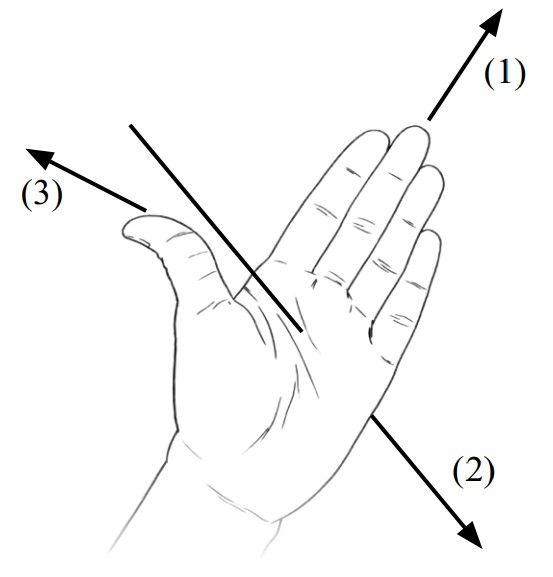
\includegraphics[scale=0.3]{figs/VN12-Y24-PH-SYL-025P-3}}
	\loigiai{}
\end{ex}
% ===================================================================
\begin{ex}
	\immini{
		Một vòng dây phẳng có dạng hình tròn đặt trong không khí, bán kính $\SI{10}{\centi\meter}$, bên trong có dòng điện chạy qua với cường độ $I_1=\SI{2.0}{\ampere}$. Một đoạn dây dẫn thẳng AB mang dòng điện có cường độ $I_2=\SI{1.0}{\ampere}$ đặt xuyên qua tâm khung dây và vuông góc với mặt phẳng khung dây như hình bên. Lực từ tác dụng lên đoạn dây có độ lớn
		\choice
		{\True $\SI{0}{\newton}$}
		{$\SI{0.2}{\newton}$}
		{$\SI{0.4}{\newton}$}
		{$\SI{8E-5}{\newton}$}
	}
	{
		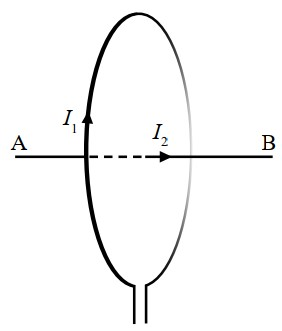
\includegraphics[scale=0.5]{figs/VN12-Y24-PH-SYL-025P-4}
	}
	\loigiai{}
\end{ex}
% ===================================================================
\begin{ex}
	\immini{Đoạn dây AB có khối lượng $m$ và độ dài $\ell$; hai lò xo giống hệt nhau và có cùng độ cứng $k$ được bố trí như hình bên. Nếu độ dãn của hai lò xo tăng từ $x_0$ đến $x$ khi có dòng điện cường độ $I$ chạy từ B sang A thì cảm ứng từ có độ lớn bằng
		\choice
		{$\dfrac{m g}{I \ell}$}
		{$\dfrac{m g x}{I \ell}$}
		{$\dfrac{m g I}{\ell x_0}$}
		{\True $\dfrac{m g}{I \ell}\left(\frac{x-x_0}{x_0}\right)$}
	}
	{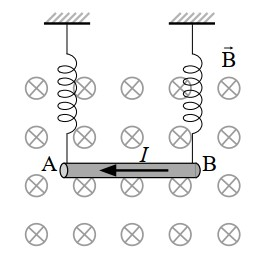
\includegraphics[scale=0.65]{figs/VN12-Y24-PH-SYL-025P-5}}
	\loigiai{}
\end{ex}
% ===================================================================
\begin{ex}
	\immini{
		Một vòng dây dẫn hình tròn nhỏ được treo lơ lửng bởi một sợi dây cách điện. Một vòng dây dẫn khác đồng trục với vòng dây nhỏ, mang dòng điện $I$, dịch chuyển đến gần vòng dây nhỏ như hình bên. Vòng dây nhỏ sẽ
		
		\choice
		{bị hút về phía vòng dây lớn}
		{\True bị đẩy bởi vòng dây lớn}
		{không chịu tác dụng của lực nào}
		{đứng yên}
	}
	{
		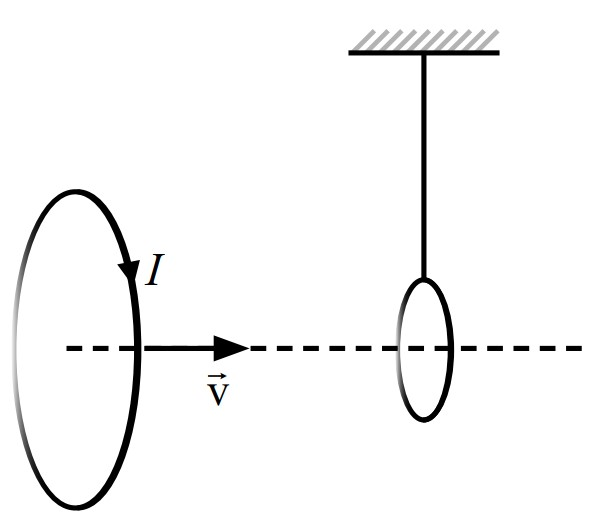
\includegraphics[scale=0.4]{figs/VN12-Y24-PH-SYL-025P-6}
	}
	
	\loigiai{}
\end{ex}
% ===================================================================
\begin{ex}
	Một khung dây dẫn quay xung quanh một trục trong một mặt phẳng vuông góc với các đường sức của một từ trường đều với tốc độ góc không đổi. Đồ thị nào dưới đây biểu diễn sự phụ thuộc thời gian của suất điện động cảm ứng xuất hiện trong khung?
	\choice
	{\True 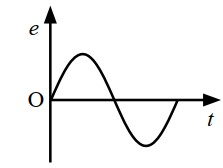
\includegraphics[width=0.35\linewidth]{figs/VN12-Y24-PH-SYL-025P-7A}}
	{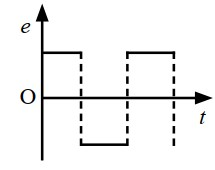
\includegraphics[width=0.35\linewidth]{figs/VN12-Y24-PH-SYL-025P-7B}}
	{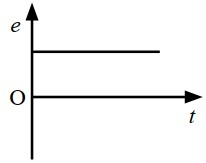
\includegraphics[width=0.35\linewidth]{figs/VN12-Y24-PH-SYL-025P-7C}}
	{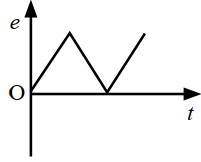
\includegraphics[width=0.35\linewidth]{figs/VN12-Y24-PH-SYL-025P-7D}}
	\loigiai{}
\end{ex}
% ===================================================================
\begin{ex}
	Một khung dây phẳng gồm $N$ vòng dây, tiết diện hình tròn có bán kính $r$. Khung dây được đặt trong một từ trường đều có vector cảm ứng $\vec{B}$ vuông góc với mặt phẳng tiết diện của nó. Từ thông qua khung dây được xác định bởi biểu thức nào sau đây?
	\choice
	{\True $N B \pi r^2$}
	{$\dfrac{1}{2} N B \pi r^2$}
	{$B \pi r^2$}
	{$\dfrac{1}{2} B \pi r^2$}
	\loigiai{}
\end{ex}
% ===================================================================
\begin{ex}
	\immini{
	Từ thông gửi qua mặt giới hạn của một khung dây dẫn được đặt trong từ trường có giá trị biến thiên theo thời gian được mô tả trong đồ thị ở hình bên. Suất điện động cảm ứng xuất hiện trong khung dây có độ lớn cực đại là
	\choice[2]
	{$\SI{5}{\volt}$}
	{$\SI{10}{\volt}$}
	{\True $\SI{8.75}{\volt}$}
	{$\SI{4.16}{\volt}$}
	}
	{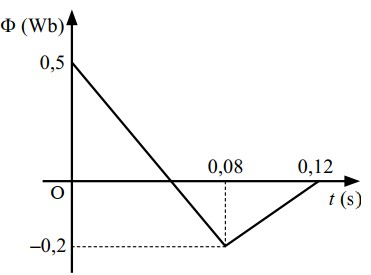
\includegraphics[scale=0.7]{figs/VN12-Y24-PH-SYL-025P-8}}
	\loigiai{}
\end{ex}
% ===================================================================
\begin{ex}
	Nội dung nào sau đây về mô hình sóng điện từ là \textbf{không} chính xác?
	\choice
	{Từ trường biến thiên theo thời gian làm xuất hiện điện trường xoáy trong không gian}
	{Điện trường biến thiên làm xuất hiện từ trường biến thiên}
	{Điện từ trường lan truyền trong không gian gọi là sóng điện từ}
	{\True Sóng điện từ không truyền được trong chân không}
	\loigiai{}
\end{ex}
% ===================================================================
\begin{ex}
	Thiết bị nào sau đây chỉ hoạt động với dòng điện xoay chiều?	
	\choice
	{Bóng đèn}
	{Động cơ điện}
	{\True Máy biến áp}
	{Chuông điện}
	\loigiai{}
\end{ex}
% ===================================================================
\begin{ex}
	\immini{
	Một cuộn dây phẳng, hình chữ nhật được đặt giữa hai cực của nam châm. Cho dòng điện đi qua cuộn dây thì cuộn dây quay xung quanh trục của nó theo chiều như hình dưới.\\
	Điều nào sau đây sẽ làm cho cuộn dây quay theo chiều ngược lại?
	\choice
	{Giảm cường độ dòng điện đi qua cuộn dây}
	{Tăng số vòng dây quấn của cuộn dây}
	{\True Đảo chiều của dòng điện đi qua cuộn dây}
	{Đảo chiều của dòng điện đi qua cuộn dây, đồng thời đảo hai cực của nam châm}
	}
	{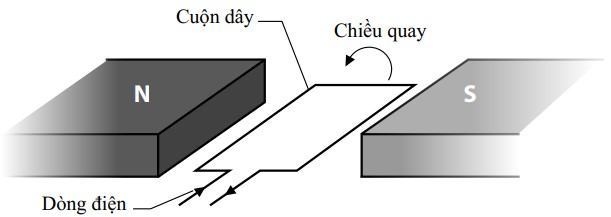
\includegraphics[scale=0.6]{figs/VN12-Y24-PH-SYL-025P-9}}
	\loigiai{}
\end{ex}

% ===================================================================
\begin{ex}
	Một dòng điện xoay chiều có cường độ phụ thuộc thời gian theo phương trình: $i=\xsi{2 \cos (100 \pi t)}{\ampere}$. Trong giây đầu tiên kể từ gốc thời gian $(t=0)$, dòng điện này đổi chiều bao nhiêu lần?
	\choice
	{2}
	{50}
	{\True 100}
	{99}
	\loigiai{}
\end{ex}

\Closesolutionfile{ans}
\subsection{Câu trắc nghiệm đúng/sai}
\textit{Thí sinh trả lời từ câu 1 đến câu 4. Trong mỗi ý \textbf{a)}, \textbf{b}, \textbf{c)}, \textbf{d)} ở mỗi câu, thí sinh chọn đúng hoặc sai}
\setcounter{ex}{0}
\Opensolutionfile{ans}[ans/VN12-Y24-PH-SYL-024-TF]
% ===================================================================
\begin{ex}
	Theo lí thuyết cổ điển, mô hình nguyên tử hydrogen gồm electron quay quanh hạt nhân trên quỹ đạo tròn có bán kính $\SI{5.3E-11}{\meter}$ với tốc độ $v$.	
	\begin{center}
		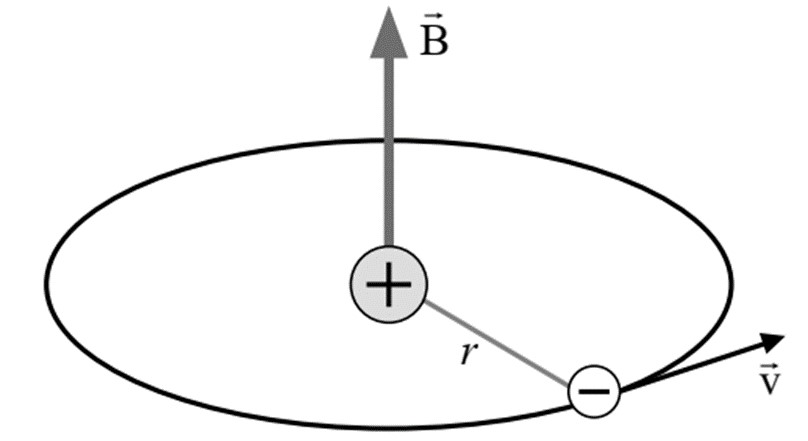
\includegraphics[width=0.3\linewidth]{figs/VN12-Y24-PH-SYL-025P-10}
	\end{center}
	\choiceTF[t]
	{\True Sự chuyển động của electron quanh hạt nhân tạo nên một dòng điện tròn}
	{\True Tốc độ của electron không phụ thuộc vào chuyển động nhiệt của nguyên tử hydrogen}
	{Chiều của vector cảm ứng từ do dòng điện này tạo ra tại tâm của nguyên tử được biểu diễn như hình bên}
	{\True Độ lớn cảm ứng từ do dòng điện này gây ra tại vị trí hạt nhân có giá trị không đổi}
	\loigiai{}
\end{ex}
% ===================================================================
\begin{ex}
	Một đoạn dây dẫn MN có khối lượng $m$, độ dài $L$, mang dòng điện $I$, được giữ lơ lửng trong một mặt phẳng nằm ngang nhờ một từ trường đều có các đường sức từ hợp một góc $\theta$ với đoạn dây và cũng nằm trong mặt phẳng nằm ngang như hình sau.
	\begin{center}
		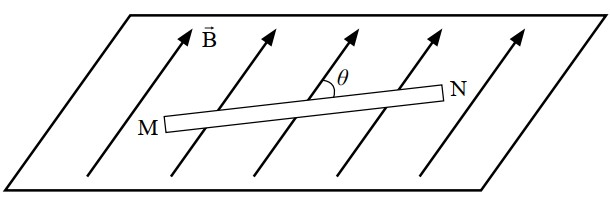
\includegraphics[width=0.4\linewidth]{figs/VN12-Y24-PH-SYL-025P-11}
	\end{center}	
	\choiceTF[t]
	{\True Dòng điện qua đoạn dây có chiều từ M sang N}
	{\True Cường độ dòng điện qua đoạn dây là $I=\dfrac{m g}{B L \sin \theta}$}
	{Khi đoạn dây quay tròn trong mặt phẳng nằm ngang thì lực từ tác dụng lên nó có độ lớn không đổi}
	{\True Nếu đồng thời đổi chiều của các đường sức từ và chiều dòng điện thì lực từ tác dụng lên đoạn dây vẫn có chiều như cũ}
	\loigiai{}
\end{ex}
% ===================================================================
\begin{ex}
	Một nam châm nhỏ $M$ được thả rơi xuyên qua một vòng dây $R$ lắp cố định. Gọi $g$ là gia tốc rơi tự do.
	\begin{center}
		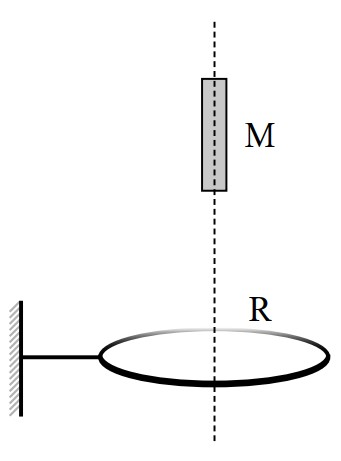
\includegraphics[width=0.2\linewidth]{figs/VN12-Y24-PH-SYL-025P-12}
	\end{center}
	\choiceTF[t]
	{Gia tốc của vật $M$ sẽ lớn hơn $g$ khi nó ở phía trên $R$ và đang chuyển động về phía $R$}
	{\True Gia tốc của vật $M$ sẽ nhỏ hơn $g$ khi nó ở phía dưới $R$ và đang chuyển động ra xa $R$}
	{\True Khi nam châm $M$ đang rơi, trong vòng dây xuất hiện suất điện động cảm ứng}
	{Khi nam châm $M$ đang rơi, dòng điện cảm ứng xuất hiện trong vòng dây $R$ có chiều kim đồng hồ khi nhìn từ trên xuống}
	\loigiai{}
\end{ex}
% ===================================================================
\begin{ex}
	Dòng điện do một máy phát điện tạo ra có cường độ biến theo thời gian được cho trong hình bên.	
	\begin{center}
		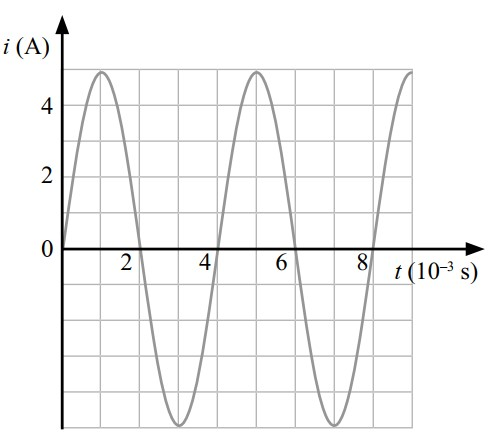
\includegraphics[width=0.4\linewidth]{figs/VN12-Y24-PH-SYL-025P-13}
	\end{center}
	\choiceTF[t]
	{\True Dòng điện được tạo ra là dòng điện xoay chiều}
	{Chu kì của dòng điện là $\SI{4}{\second}$}
	{\True Cường độ dòng điện hiệu dụng có giá trị $\xsi{\dfrac{5\sqrt{2}}{2}}{\ampere}$}
	{\True Phương trình của dòng điện là: $
		i=\xsi{5 \cos \left(500 \pi t-\dfrac{\pi}{2}\right)}{\left(\ampere\right)}$}
	\loigiai{}
\end{ex}

\Closesolutionfile{ans}
\subsection{Câu trắc nghiệm trả lời ngắn} \textit{Thí sinh trả lời từ câu 1 đến câu 6}
\setcounter{ex}{0}
\Opensolutionfile{ans}[ans/VN12-Y24-PH-SYL-024-TL]
% ===============================================================
\begin{ex}
	Trong một thí nghiệm đo cảm ứng từ bằng phương pháp cân "dòng điện" với chiều dài tương đương đoạn dây dẫn đặt trong từ trường của nam châm là 10 m và góc $\theta=\SI{90}{\degree}$, người ta thu được kết quả như sau:
	\begin{center}
		\begin{tabular}{|M{2cm}|M{5cm}|M{5cm}|}
			\hline \thead{Lần đo} & \thead{Cường độ dòng điện $\left(\si{\ampere}\right)$} & \thead{Lực từ $\left(\si{\newton}\right)$} \\
			\hline 1 & 0,1 & 0,02 \\
			\hline 2 & 0,2 & 0,05 \\
			\hline 3 & 0,3 & 0,07 \\
			\hline
		\end{tabular}
	\end{center}
	Giá trị trung bình của độ lớn cảm ứng từ trong thí nghiệm trên là bao nhiêu $\si{\tesla}$? \textit{(Kết quả làm tròn đến chữ số hàng phần trăm.)}
	\shortans[oly]{ 0,02}
	\loigiai{
		
	}
\end{ex}
% ===============================================================
\begin{ex}
	Một đoạn dây dẫn thẳng có khối lượng trên đơn vị độ dài là $\SI{0.5}{\gram/\centi\meter}$ mang dòng điện $\SI{2}{\ampere}$ chạy trên phương ngang. Cần một từ trường có có độ lớn tối thiểu bằng bao nhiêu $\si{\tesla}$ để giữ cho sợi dây này không rơi xuống? Lấy $g=\SI{10}{\meter/\second^2}$. \textit{(Kết quả làm tròn đến chữ số hàng phần trăm.)}
	\shortans[oly]{0,25 }
	\loigiai{
		
	}
\end{ex}
% ===============================================================
\begin{ex}
	\immini{
		Một vòng dây tròn tiết diện $\SI{20}{\centi\meter^2}$ được lắp một trục thẳng đứng và quay tròn xung quanh trục đó với tốc độ góc $\omega$ không đổi trong một từ trường đều $B=\SI{0.05}{\tesla}$ có các đường sức từ vuông góc với trục quay của vòng dây (hình bên). 
		Từ thông cực đại qua vòng dây là bao nhiêu $\si{\milli\weber}$? \textit{(Kết quả làm tròn đến chữ số hàng phần mười.)}
	}
	{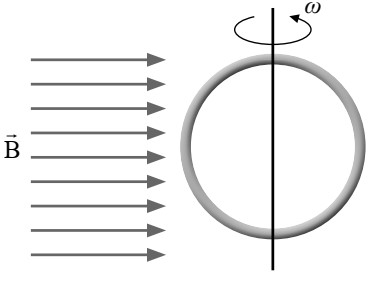
\includegraphics[scale=0.4]{figs/VN12-Y24-PH-SYL-025P-14}}
	\shortans[oly]{0,1}
	\loigiai{
		
	}
\end{ex}
% ===============================================================
\begin{ex}
	Một khung dây phẳng có diện tích tiết diện $\SI{40}{\centi\meter^2}$, gồm 800 vòng dây. Trong khoảng thời gian $\SI{1.0}{\milli\second}$, khung dây quay từ vị trí có mặt phẳng khung dây vuông góc với các đường sức từ đến vị trí có mặt phẳng khung dây song song với các đường sức từ của một từ trường đều có độ lớn $\SI{5.0E-4}{\tesla}$. Độ lớn suất điện động cảm ứng trung bình xuất hiện trong khung dây là bao nhiêu $\si{\volt}$? \textit{(Kết quả làm tròn đến chữ số hàng phần mười.)}
	\shortans[oly]{1,6}
	\loigiai{
		
	}
\end{ex}
% ===============================================================
\begin{ex}
	Trong thiên văn học, người ta có thể lập bản đồ các đám mây khí hydrogen trong vũ trụ bằng cách dò tìm sóng điện từ có bước sóng $\SI{21}{\centi\meter}$ do những đám mây này phát ra và lan truyền trong không gian. Tần số của sóng điện từ này là bao nhiêu $\si{\giga\hertz}$? \textit{(Kết quả làm tròn đến chữ số hàng phần trăm.)}
	\shortans[oly]{1,43}
	\loigiai{
		
	}
\end{ex}
% ===============================================================
\begin{ex}
	Cho một dòng điện xoay chiều $i=\xsi{4 \sqrt{2} \cos \left(100 \pi t+\dfrac{\pi}{4}\right)}{\left(\ampere\right)}$ đi qua một vật dẫn có điện trở không đổi $R=\SI{1200}{\ohm}$. Nhiệt lượng toả ra bởi dòng điện trên vật dẫn trong thời gian 15 phút là bao nhiêu $\si{\mega\joule}$? \textit{(Kết quả làm tròn đến chữ số hàng phần mười.)}
	\shortans[oly]{17,3}
	\loigiai{
		
	}
\end{ex}
\Closesolutionfile{ans}